%% General definitions
\documentclass{article} %% Determines the general format.
\usepackage{a4wide} %% paper size: A4.
\usepackage[utf8]{inputenc} %% This file is written in UTF-8.
%% Some editors on Windows cannot save files in UTF-8.
%% If there is a problem with special characters not showing up
%% correctly, try switching "utf8" to "latin1" (ISO 8859-1).
\usepackage[T1]{fontenc} %% Format of hte resulting PDF file.
\usepackage{fancyhdr} %% Package to create a header on each page.
\usepackage{lastpage} %% Used for "Page X of Y" in the header.
											%% For this to work, you have to call pdflatex twice.
\usepackage{enumerate} %% Used to change the style of enumerations (see below).

\usepackage{amssymb} %% Definitions for math symbols.
\usepackage{amsmath} %% Definitions for math symbols.
\usepackage{amsthm}
\usepackage{braket}
\usepackage{graphicx}
\usepackage{float}

\usepackage{tikz}  %% Pagacke to create graphics (graphs, automata, etc.)
\usetikzlibrary{automata} %% Tikz library to draw automata
\usetikzlibrary{arrows}   %% Tikz library for nicer arrow heads


%% Left side of header
\lhead{\course\\\semester\\Exercise \homeworkNumber}
%% Right side of header
\rhead{\authorname\\Page \thepage\ of \pageref{LastPage}}
%% Height of header
\usepackage[headheight=36pt]{geometry}
%% Page style that uses the header
\pagestyle{fancy}

\newcommand{\authorname}{Nico Bachmann\\Ruben Hutter}
\newcommand{\semester}{Spring semester 2023}
\newcommand{\course}{Theory of Computer Science}
\newcommand{\homeworkNumber}{2}


\begin{document}

\section*{Exercise \homeworkNumber.1}
We did the tutorial, but are so kind to only upload the pdf without all the
.jff files ;)

\section*{Exercise \homeworkNumber.2}
\begin{enumerate}[(a)]
	\item
	This is the graphical representation of the DFA $M = \left \langle
		\set{q_0, q_1, q_2, q_3}, \set{a, b}, \delta,\; q_0, \set{q_2}
		\right \rangle$.
	\begin{figure}[H]
		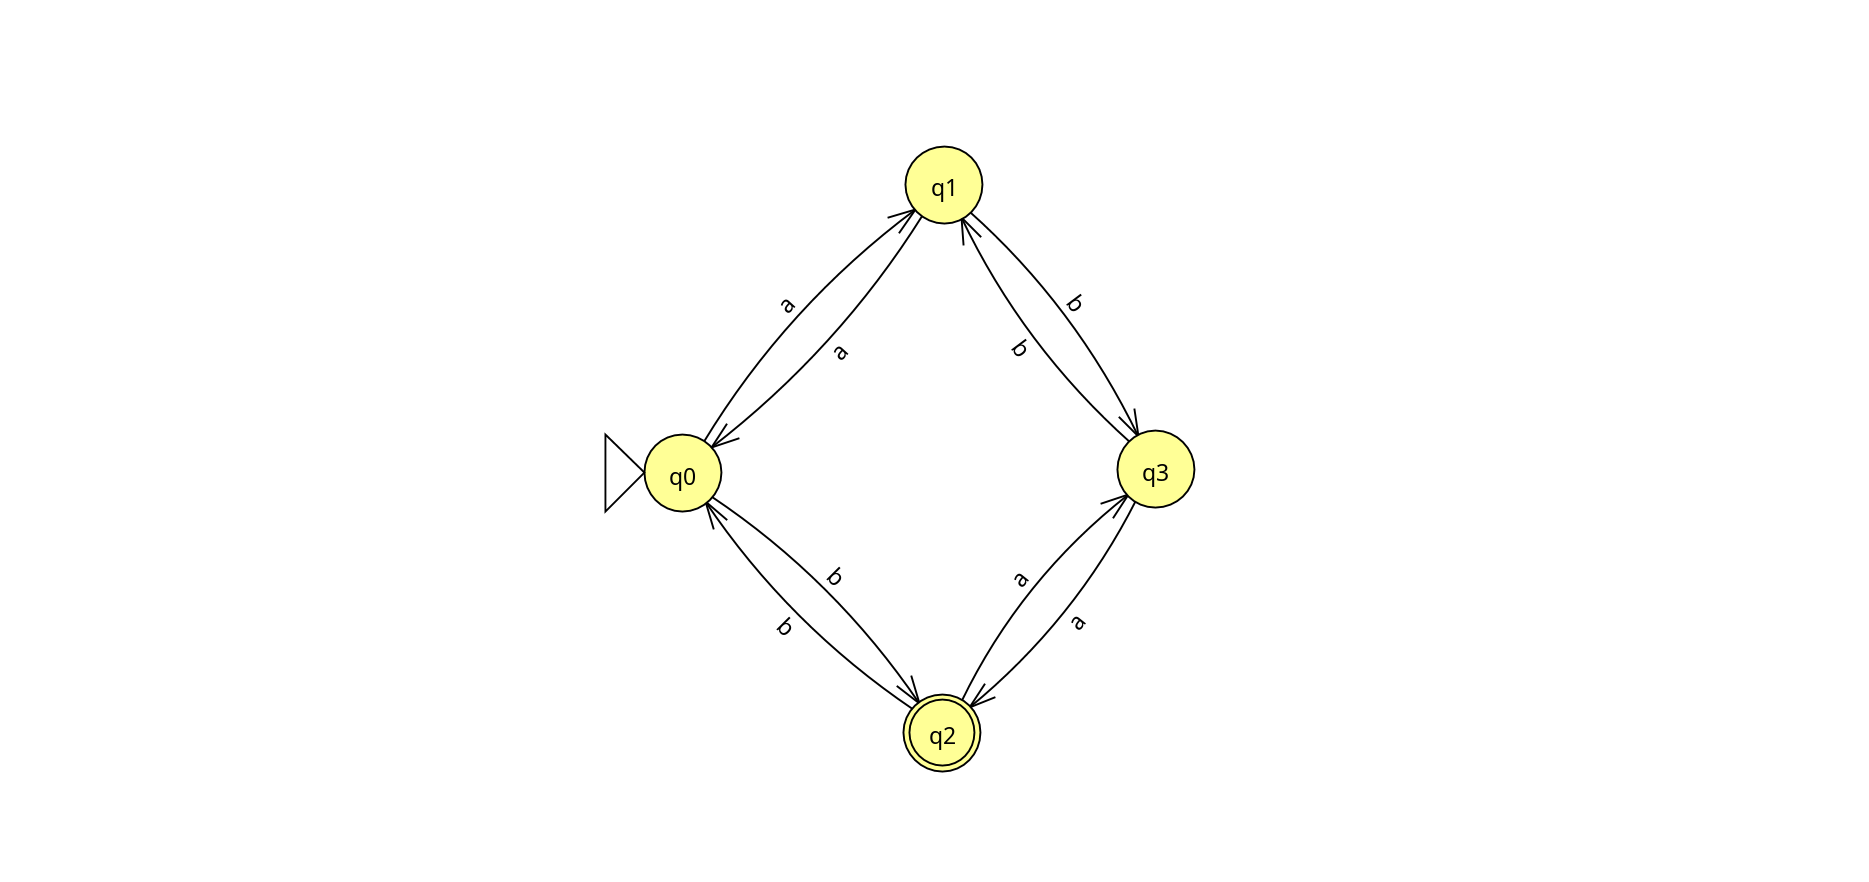
\includegraphics[width=\linewidth]{ex2a.png}
		\centering
		\caption{Graphical representation of DFA $M$}
	\end{figure}

	\item
	For the sequence "abbab", we visit the following states:
	$$
	q_0 \to q_1 \to q_3 \to q_1 \to q_0 \to q_2
	$$
	As you can see, we end up at $q_2$ which is actually one, and the only, final state of the DFA $M$.

	\item
	$M$ recognizes every language that has an odd number of "b"'s in it (at least one) and that has 0 or
	an even number of "a"'s. So the minimal length of the words of the language has to be 1, since you have to reach $q_2$ from $q_0$.

\end{enumerate}

\clearpage

\section*{Exercise \homeworkNumber.3}
\begin{figure}[H]
	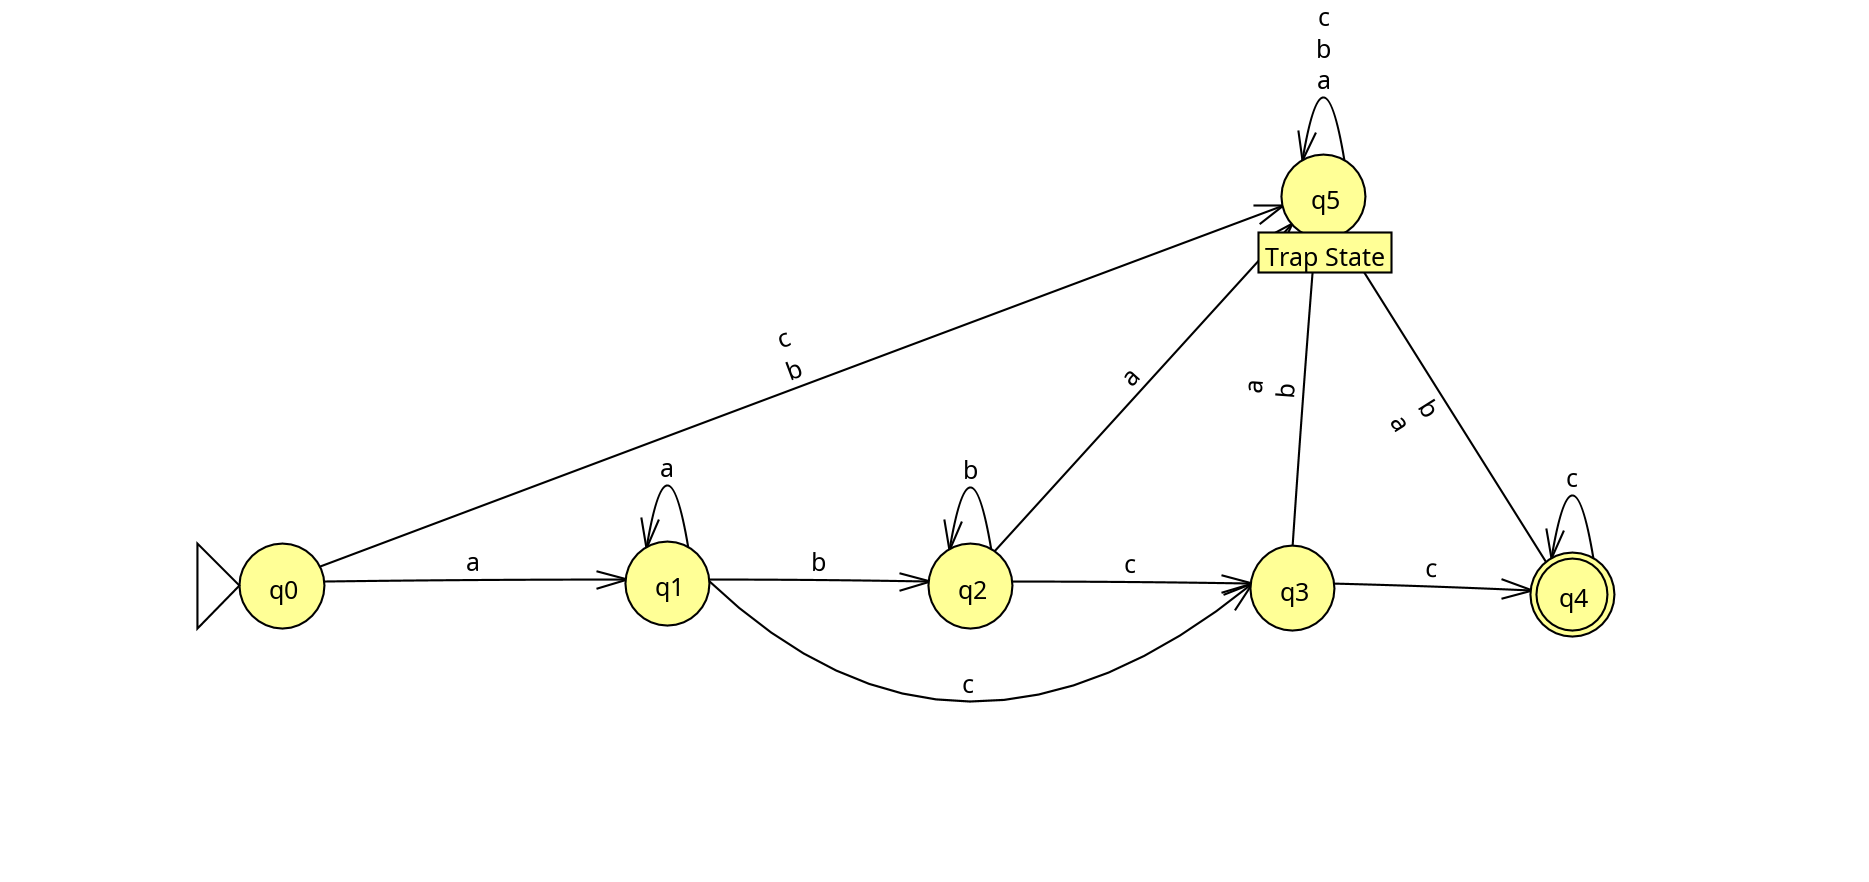
\includegraphics[width=\linewidth]{ex3.png}
	\centering
	\caption{The DFA for the language $L = \set{a^x \, b^y \, c^z \mid x \ge 1,\; y \ge 0,\; z \ge 2}$}
\end{figure}

\clearpage

\section*{Exercise \homeworkNumber.4}
\begin{enumerate}[(a)]
	\item
	Yes, because if we follow the states given by the word 0101010 we end up at
	$q_2$, which is a final state of the NFA.
	
	After the first 0 we end up at $q_2$, from which we can go back to $q_0$ (with $\epsilon$) and then
	go to $q_1$ with 1. The following elements 010 we do by staying on $q_1$; then we go to $q_2$ with 1
	and we end on $q_2$ with the last 0 passing by $q_0$.

	\item
	This is the DFA equivalent to the NFA on the Exercise sheet:
	\begin{figure}[H]
		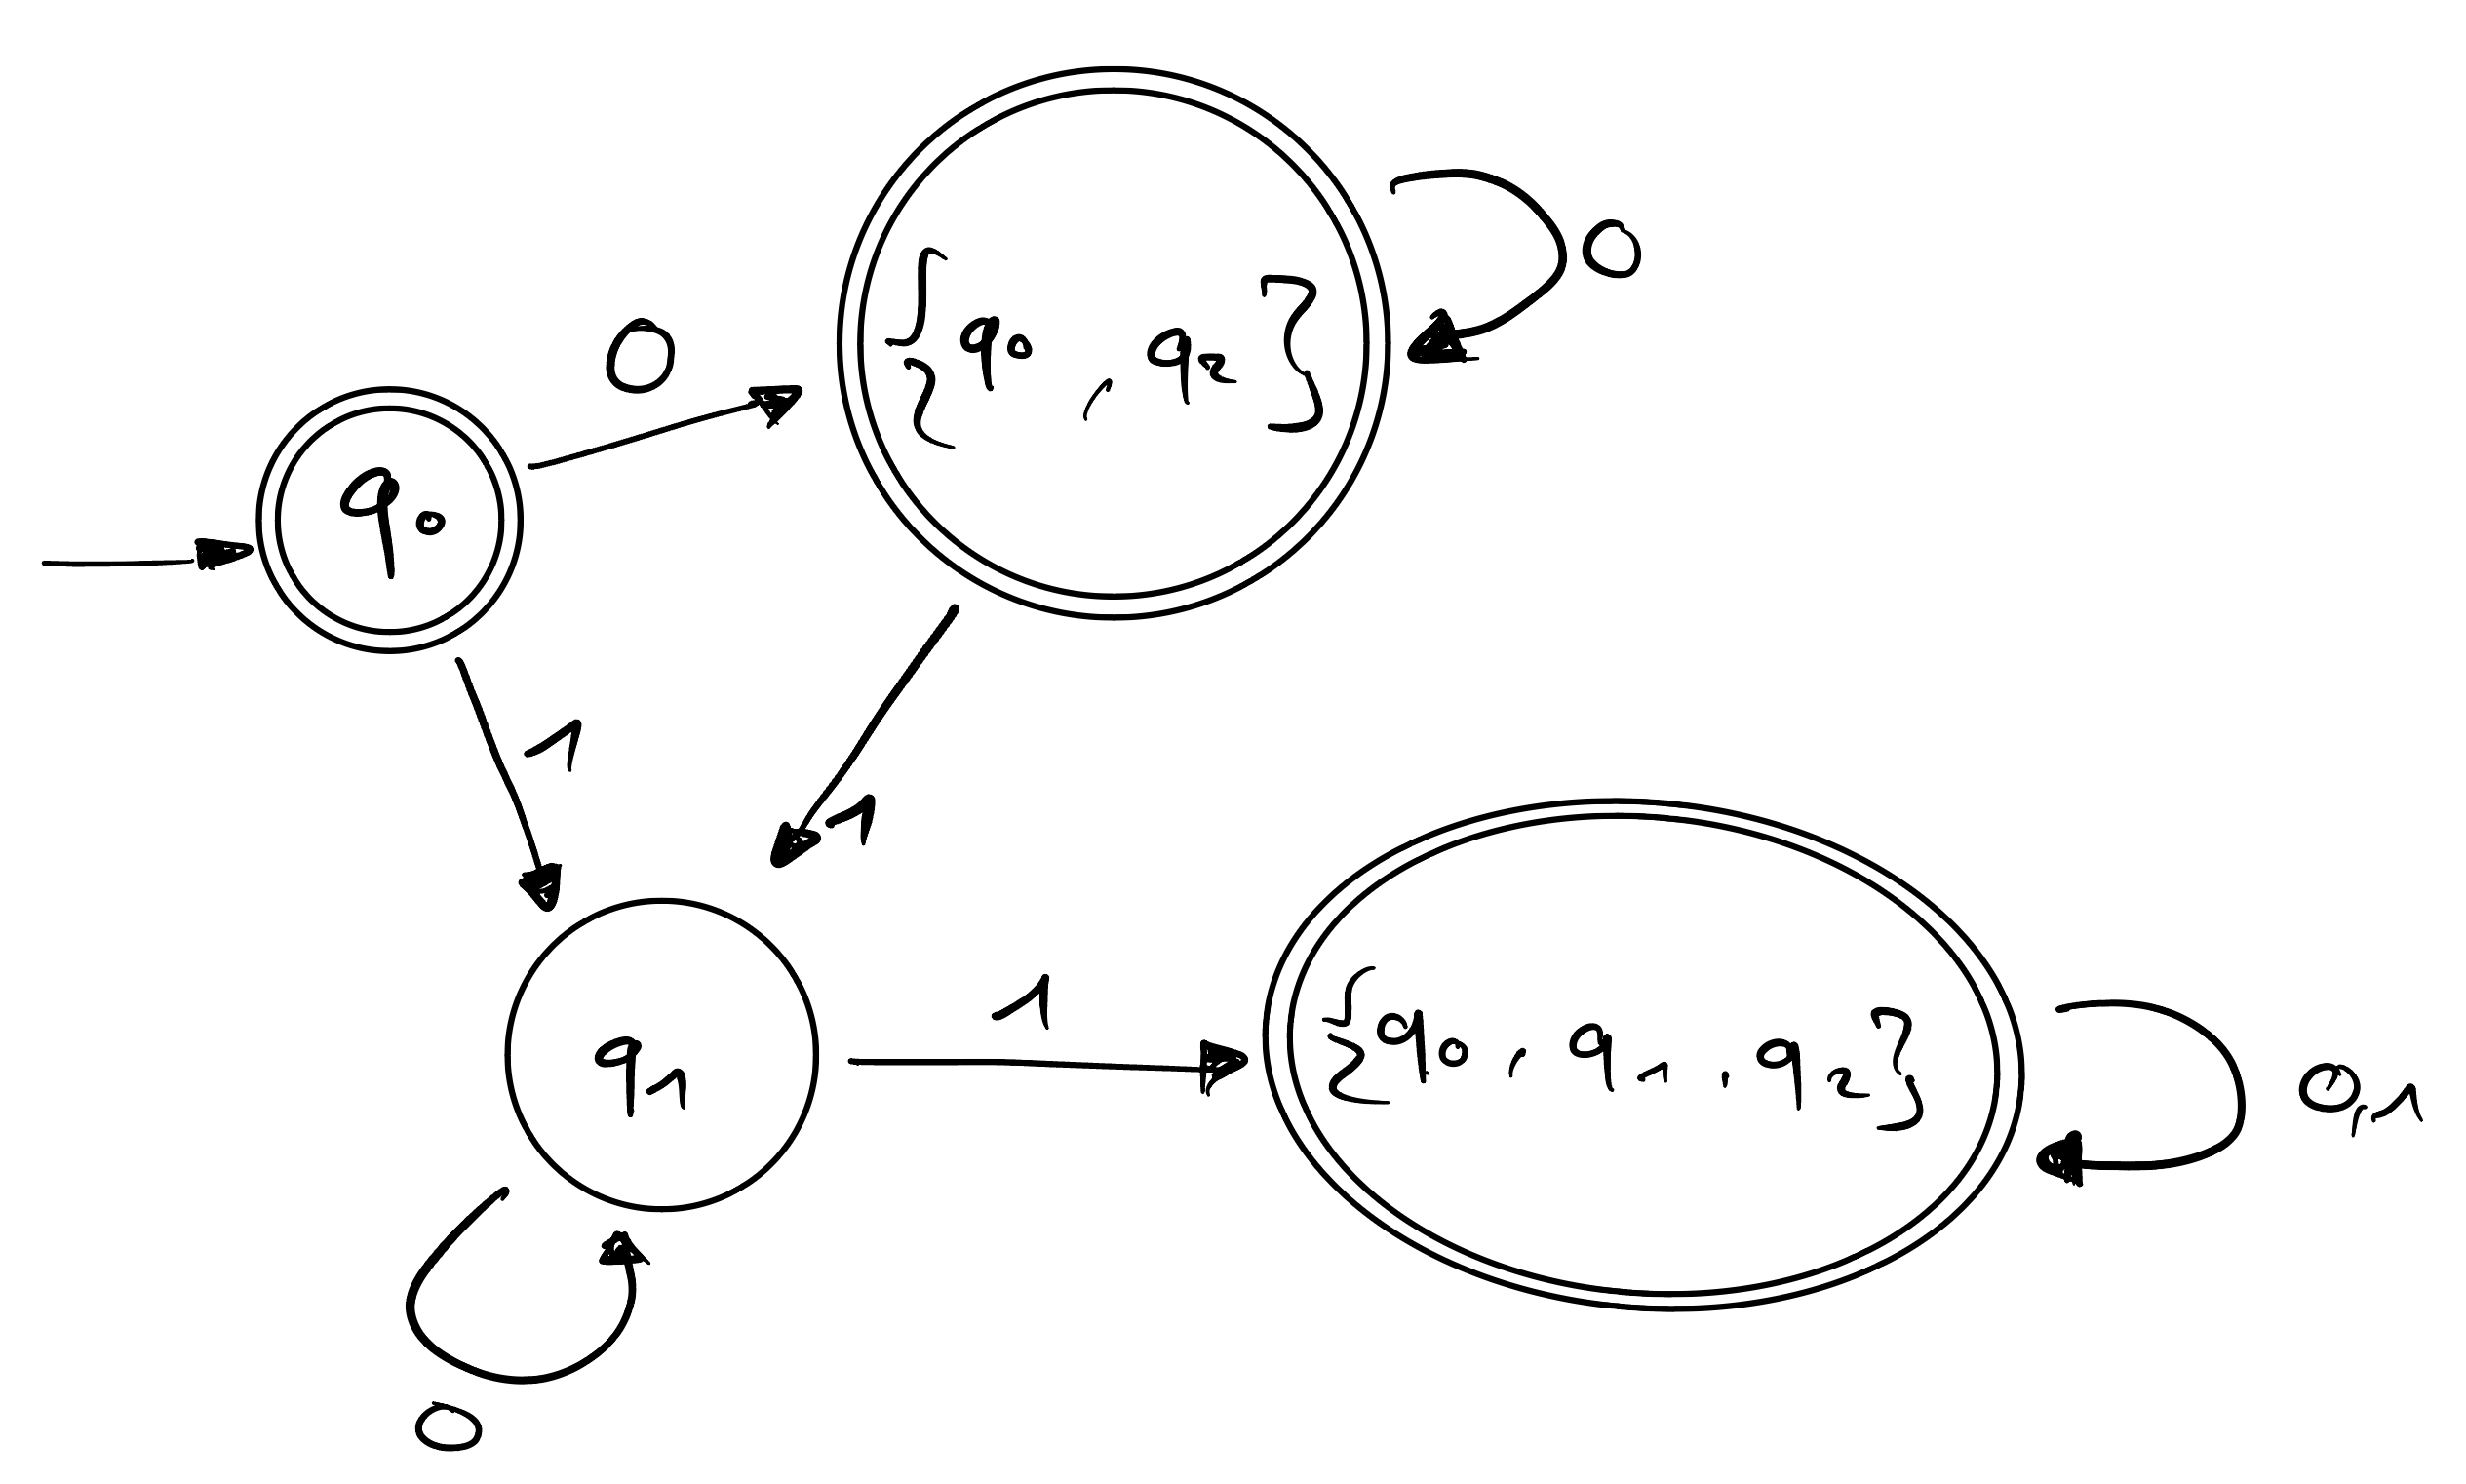
\includegraphics[width=\linewidth]{ex4b.png}
		\centering
		\caption{DFA}
	\end{figure}
\end{enumerate}

\end{document}
